
\chapter{Soundings: UML Sequence diagrams}
\label{artifact}

Class diagrams are the bread-and-butter of UML. They depict the static
features of software systems: the classes, methods, and associations that
connect them. Complementary to class diagrams are another type of UML
artifact\footnote{By the way, the term \textbf{artifact} in software
engineering means ``a document, diagram, computer program, or some other
tangible deliverable that results from carrying out a development activity.''
The measurable progress a development team makes consists of the various
artifacts they produce along the way.} called \textbf{sequence diagrams}. They
show the \textit{dynamic} interrelations between objects as a system's code
executes.

Each sequence diagram depicts one scenario, or flow through the system. Unlike
a class diagram, which is sort of ``always true'' and shows all the permanent
and unvarying features of the program in question, every sequence diagram
shows its own path: its own thread of execution in a particular, hypothetical
scenario. After all, nearly every time you run a program, something different
happens, either because the user makes different choices, network and system
latencies cause various tasks to end at different times, or a random number
generator is involved. A sequence diagram selects just \textit{one} possible
outcome and highlights it start-to-finish so that an example of how the
classes are intended to interact is unveiled.

I think of a sequence diagram as a ``sounding'' in the nautical sense. In
ancient times, ship captains who suspected they were approaching land would
test how deep the water was by probing it with a sounding line. Modern ships
do the equivalent with sonar. A sounding is an exploratory investigation down
one possible path through the water's depths to see what's below. One sounding
doesn't tell you everything about the whole region's topography, but it tells
you a great deal about the specific area you're in. And if you perform several
soundings, you can combine the clues you obtain from each one to build a
mental picture of a wider section of the ocean floor. A programmer can do the
same by learning from several different sequence diagrams, each of which
tells a different story.

Sequence diagrams are designed to be perused in conjunction with their
corresponding class diagrams. I always tell students: ``when you look at a
sequence diagram, only look at it with one eyeball; keep the other eyeball on
the class diagram.'' As we'll see, both diagrams have to be ``in sync'' with
each other, since information presented on one must be compatible with what's
on the other.

\section{Going backwards}

\vspace{-.2in}
{\large \textbf{Reverse-engineering a sequence diagram from code}}

Flip back to Figure~\ref{fig:fullClassDiag} from chapter~\ref{ch:blueprints}
(p.~\pageref{fig:fullClassDiag}). This is our baseball simulator example. Keep
your finger in this page for reference as you follow along in this section.

We're going to begin our ``sounding'' through this program by starting in the
\texttt{Simulator} class's \texttt{.printAllStars()} method. Its job is to
print out the names of the teams and their all-time greatest hitters, like
this:

\begin{Verbatim}[fontsize=\normalsize,samepage=true,frame=single]
  NY Yankees - Babe Ruth (3)
  St. Louis Cardinals - Stan Musial (6)
  NY Giants - Willie Mays (24)
  Milwaukee Braves - Hank Aaron (44)
  Boston Red Sox - Ted Williams (9)
  ...
\end{Verbatim}

The story told by a sequence diagram has to begin somewhere; this is
sometimes, but not always, in \texttt{main()}. Here we pick up the action in
\texttt{.printAllStars()}. Let's say the code for it looked like this:

\begin{Verbatim}[fontsize=\small,samepage=true,frame=single]
class Simulator {
    ...
    public void printAllStars() {
        int numTeams = teams.size();
        for (int i=0; i<numTeams; i++) {
            Team nextTeam = teams.get(i);
            System.out.println(nextTeam + " - " nextTeam.getBestHitter());
        }
    }
}
\end{Verbatim}

Normally, we \textit{start} with a UML design and then write the code to
implement it; but here, we're going to reverse-engineer the UML sequence
diagram \textit{from} the code. This is simply because you've seen a lot more
code than sequence diagrams in your life, and I think you'll better understand
how sequence diagrams work if I show it to you this way first. (In the next
section we'll go the other way.)

\begin{figure}
\centering
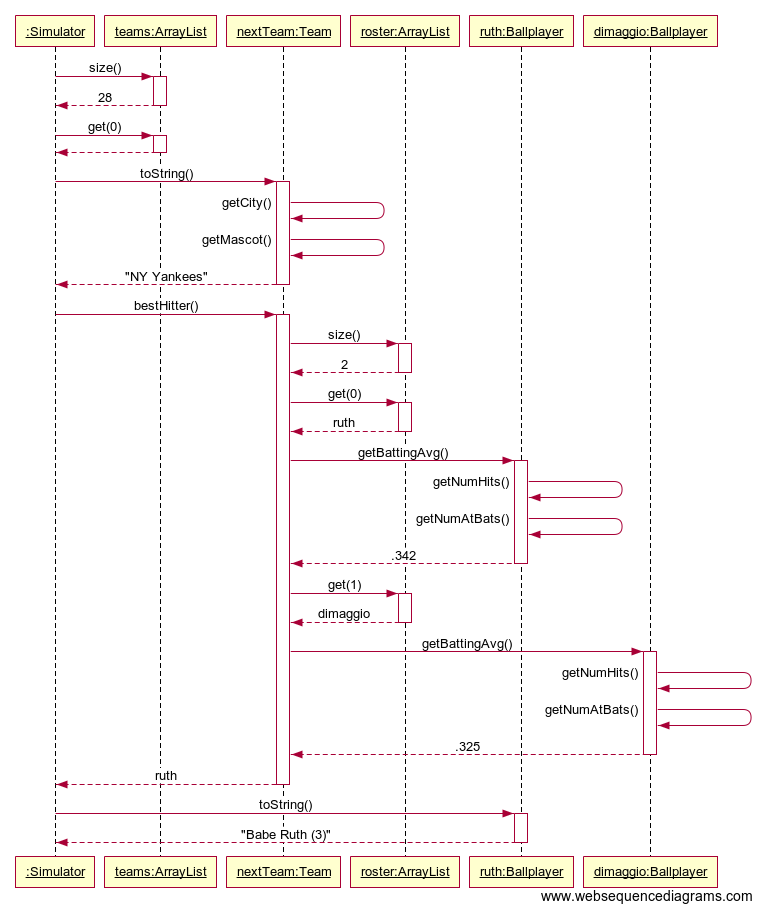
\includegraphics[width=1.1\textwidth]{baseballSeqDiag.pdf} % 1056x1180
\vspace{.1in}
\caption{A sequence diagram: Baseball example.}
\label{fig:baseballSeqDiag}
\end{figure}

\subsection{Sequence diagram features}

Now look at the enormous diagram in Figure~\ref{fig:baseballSeqDiag}. To get
your bearings, note these two important aspects of sequence diagrams:

\begin{compactitem}
\item The \textbf{\textit{objects}} (and occasionally classes) that
participate in this scenario \textbf{\textit{appear across the top}} of the
diagram. There is no inherent meaning to the order in which they appear, but
often objects that are involved earlier in the code path are on the left side.
\item The dashed line that extends down the page from each box ``goes with''
that object. Horizontal arrows that originate from (or point to) that line are
methods that object calls (or that are called on it).
\item \textit{\textbf{Time goes down.}} In other words, as the code path
executes in time, we move progressively further down the page.
\end{compactitem}

\subsection{What the arrows mean}

So we begin by looking at the upper-left corner, where the top-most arrow goes
from the ``\texttt{:Simulator}'' box to the ``\texttt{teams:ArrayList}'' box,
and is labeled ``\texttt{size()}''. As I'm sure you can guess, this corresponds
to the line of code: ``\texttt{int numTeams = teams.size();}'' which is the
first thing we do in \texttt{.printAllStars()}.

{\huge $\star$} Here's how you interpret \textit{any} arrow on a sequence diagram:

\begin{compactenum}
\item Every arrow is a method call. (Important: method calls are the
\textit{only} part of the code that can be shown on a sequence diagram.)
\item The vertical dashed line where the arrow \textit{starts} is the object
that makes that call. (In other words, if an arrow starts from a ``:Person''
box, then somewhere in a method of the \texttt{Person} class we can expect to
find this method being called.)
\item The vertical dashed line where the arrow \textit{ends} is the object on
which the method is \textit{being} called. (In other words, if an arrow ends
on a ``:Book'' box, then we're calling the method on that \texttt{Book}
object.)
\item The writing on the arrow is the name of the method being called, plus
any parameters.
\end{compactenum}

So, that first arrow in Figure~\ref{fig:baseballSeqDiag} means:

\begin{center}
\begin{tabular}{m{.1in} m{4in}}
\huge $\star$ & \large ``Somewhere in a method of the \texttt{Simulator} class, we're calling
\texttt{.size()} on an \texttt{ArrayList} object named \texttt{teams}.''
\end{tabular}
\end{center}

(Before you go on, read that sentence, and stare at that arrow, several times
and make sure you're absolutely certain of every detail. This one key idea is
the secret to understanding sequence diagrams.)

Notice that the arrow terminates on the top of a skinny box that extends a
centimeter or so down the \texttt{teams:ArrayList}'s vertical dashed line.
This skinny box represents \textit{the time during which the program is ``in''
the \texttt{.size()} method.} It's not actually intended to specify a duration
of time (like, ``the \texttt{.size()} method will take 1.4 milliseconds to
complete'') but rather the-fact-that-it's-being-executed at all. Later, we'll
see that these skinny boxes can be (much) taller if we want our sequence
diagram to show detail about what happens \textit{inside} that method.

\subsection{Following the flow}

Okay. Let's continue down the diagram and see the rest of the action
unfolding. Keep your finger on Figure~\ref{fig:baseballSeqDiag} as we go so
you don't lose your place.

\begin{enumerate}
\itemsep.1em

\item The dashed vertical line pointing left with a ``28'' written on it is the
\textit{return value}. In this particular scenario, apparently there are 28
teams (\textit{i.e.}, 28 entries in the \texttt{ArrayList}).

\item The next call is to \texttt{.get()} the first entry in the list. Observe
how the line says literally ``\texttt{.get(0)}'' whereas the code has
``\texttt{.get(i)}'', with \texttt{i} being a loop variable. This is perfectly
fine. It means that as the code executes, the call to \texttt{ArrayList.get()}
is effectively passed the value \texttt{0} as an argument the first time it's
called, which is of course true. \textit{The fact that a loop is required is
implicit.} The designer, who created this sequence diagram, isn't spelling out
details like ``use a loop here'' for the programmer. Instead, she's
illustrating the intended pattern of method calls between objects -- the
programmer will infer the need for loops, local variables, \textit{etc.}

\item The dashed ``return value'' line is blank. That's okay too: it means the
designer didn't bother to specify a name for it. (Get used to design diagrams
containing differing levels of information in different places.)

\item Then \texttt{.toString()} is called on the returned \texttt{Team}
object. Why? Because we're \texttt{System.out.println()}'ing it, and as you'll
recall from p.~\pageref{pg:toString}, the \texttt{.toString()} method is
automatically invoked for any object that tries to be ``printed.'' So even
though our code doesn't explicitly say ``\texttt{.toString()}'' in it, the
method is nevertheless called, and is thus dutifully shown on the sequence
diagram.

\item Now play close attention. Notice that the \texttt{.toString()} arrow
isn't followed by a dashed return value arrow right away. Instead, the skinny
box extends down the page an inch or more. This is because \textit{we're
showing what's happening inside \texttt{.toString()}}. In this case, there are
two bendy arrows going from the \texttt{nextTeam:Team} line \textit{back to
itself}. These mean that the methods \texttt{.getCity()} and
\texttt{.getMascot()} are being called by the \texttt{Team} object \textit{on
itself}. This may disorient you at first, but of course there's nothing really
strange about an object calling a method on itself. After all, our
\texttt{Team.toString()} method looks like this:

\begin{Verbatim}[fontsize=\footnotesize,samepage=true,frame=single]
public class Team {
    ...
    public String toString() {
        return this.getCity() + " " + this.getMascot();
    }
    ...
    private String getCity() { return this.city; }
    private String getMascot() { return this.mascot; }
}
\end{Verbatim}

Calling a method on ``\texttt{this}'' is exactly what's indicated by those
bendy arrows.

\item Now, finally, we get our dashed arrow back to ``\texttt{:Simulator}'',
with a return value of ``\texttt{NY Yankees}''. The control flow thus transfers
from \texttt{.toString()} back to \texttt{.printAllStars()}.

\item Next up is the \texttt{.bestHitter()} method, called later on in that
same \texttt{.println()} call. This commences an even longer skinny box,
because \texttt{.bestHitter()} has a lot to do. Here it is:

\begin{Verbatim}[fontsize=\scriptsize,samepage=true,frame=single]
public class Team {
    ...
    private Ballplayer bestHitter() {
        int numPlayers = roster.size();
        Ballplayer best = roster.get(0);
        for (int i=0; i<numPlayers; i++) {
            Ballplayer b = roster.get(i);
            if (b.getBattingAvg() > best.getBattingAvg()) {
                best = b;
            }
        }
        return best;
    }
    ...
}
\end{Verbatim}

You can see that after getting the size of the roster (in this case, only two
players since this is a long enough example as it is!) we get each
\texttt{Ballplayer} in turn, ask for his batting average, and compare it to
our ``best so far'' in a typical find-the-max-element type of loop.

All of this is faithfully represented in the sequence diagram. First, the
\texttt{Team} object calls \texttt{.size()} (and gets ``2'' back). Then it
calls \texttt{.get(0)} (and gets back a player; let's say Babe Ruth), and then
calls \texttt{.getBattingAvg()} on it (getting the number .342, a jaw-dropping
lifetime average, especially for a power hitter). A moment later, it does the
same with the second player (say, Joe Dimaggio) and gets his average (still
amazing, but ``only'' .325) for comparison.

\item More detail is shown inside the calls to
\texttt{Ballplayer.getBattingAvg()}. That code looks like this:

\begin{Verbatim}[fontsize=\scriptsize,samepage=true,frame=single]
public class Ballplayer {
    ...
    public double getBattingAvg() {
        return ((double) this.getNumHits()) / this.getNumAtBats();
    }
    private String getNumHits() { return this.numHits; }
    private String getNumAtBats() { return this.numABs; }
    ...
}
\end{Verbatim}

and makes two ``self-calls'' to get this \texttt{Ballplayer}'s two relevant
statistics. Those calls are again shown as bendy loops.

\item Finally, the \texttt{Team} returns its best hitter (Babe Ruth in this
scenario) back to the \texttt{Simulator}, which again calls
\texttt{.toString()} implicitly, this time on the \texttt{Ballplayer} object.
That method returns the name of the ballplayer and his uniform number,
formatted nicely, for \texttt{Simulator.printAllStars()} to print.

\end{enumerate}

\subsection{Coming up for air}

That was a long journey through the weeds, because that sequence diagram
contained a boatload of stuff. In fact, one of the big takeaways here is that
\textit{a sequence diagram contains a ton of information about how to write
the code.}

A sequence diagram omits programming-specific details like whether to create
local variables and what to call them; whether you need a loop and what type
of loop you might choose; what the exact formula is for a computation, or the
logic to test for a condition; \textit{etc.} But it does present you with a
silver platter that says which objects of which types are intended to call
which methods on which other objects, and in what sequence.

In practice, I'd estimate that this works out to be about 70\% or so of the
decisions the programmer would otherwise have to make. What a windfall!

Before we move to our second example, let me tell you the two most common
errors I see among students trying to interpret (or create) sequence diagrams:

\begin{enumerate}
\itemsep.1em
\item \textbf{Misinterpreting what the arrowhead-side of the arrow means.}
Each arrow points to a line which represents \textit{the object on which the
method is being called.} There's a great way to sanity check this: make sure
that the class (for whatever type of object the arrow is pointing to) actually
has a method of that name!

Figure~\ref{fig:rightWrongSeqDiag} shows some common mistakes. Neither of the
top two sequence diagram fragments can possibly be correct, because they show
an \texttt{.add()} method being called on a \texttt{Review} object. Now I ask
you: look at the class diagram -- do you see an \texttt{.add()} method on the
\texttt{Review} class? Nope. That means that right away, without even thinking
any further, you can rule out the top two sequence diagram attempts in that
figure.

The bottom two versions pass this test, because in those diagram
\texttt{.add()} is being called on a \textit{\texttt{Movie}} object, which
does indeed have an \texttt{.add()} method.

\begin{figure}
\centering
\includegraphics[width=0.9\textwidth]{rightWrongSeqDiag.pdf}  %
\caption{Many wrong ways to draw the sequence diagram arrow...and one right
way.}
\label{fig:rightWrongSeqDiag}
\end{figure}

\item \textbf{Misinterpreting what the non-arrowhead-side of the arrow means.}
Each arrow originates from a line which represents \textit{the object whose
code is making the method call} (on a different object, normally). 

To sanity check this, we can't look at the class diagram alone. We have to
think about what the code looks like. Suppose this were the case:

\begin{Verbatim}[fontsize=\small,samepage=true,frame=single]
class Editor {
    ...
    public void approve(Review r, Movie m) {
        ...
        m.add(r);
    }
}
\end{Verbatim}

Even before we saw this code snippet, we already knew that \texttt{.add()}
would be called on a \texttt{Movie} object (and passed a \texttt{Review}
object as an argument) because that's in line with the class diagram. But what
we learn now is \textit{where} that line of code exists. Is it written in a
method of the \texttt{Review} class? Or the \texttt{Movie} class? Nope -- it's
in the \texttt{.approve()} method \textit{of the \texttt{Editor} class.} That
tells us that the \textit{bottom} of the four sequence diagrams in
Figure~\ref{fig:rightWrongSeqDiag} is the correct one. The third one shows a
\textit{\texttt{Review}} making the method call, but if that were the case,
the ``\texttt{m.add(r)}'' line would be somewhere in \texttt{Review.java}.

\end{enumerate}

\section{Going forwards}

\vspace{-.2in}
{\large \textbf{Using a sequence diagram to guide the implementation}}

Now normally we won't be drawing a sequence diagram after we've written the
code, although that does actually happen sometimes, like when we want to
illustrate the behavior of a system to a new member of our programming team.
(It's usually easier for them to see the diagram at a glance than it is for
them to wade through a bunch of code and try to make sense of it.)

So now we'll start with a design (both class and sequence diagram), and see
what we can infer about what the code to implement it should look like.
Figures~\ref{fig:playlistClassDiag} and \ref{fig:playlistSeq} give the
design, which you are encouraged to study in detail.

\begin{figure}
\centering
\includegraphics[width=1\textwidth]{playlistClassDiag.pdf}
\caption{The playlist program's class diagram.}
\label{fig:playlistClassDiag}

\end{figure}
\begin{figure}
\centering
%\hspace*{-1.5in}
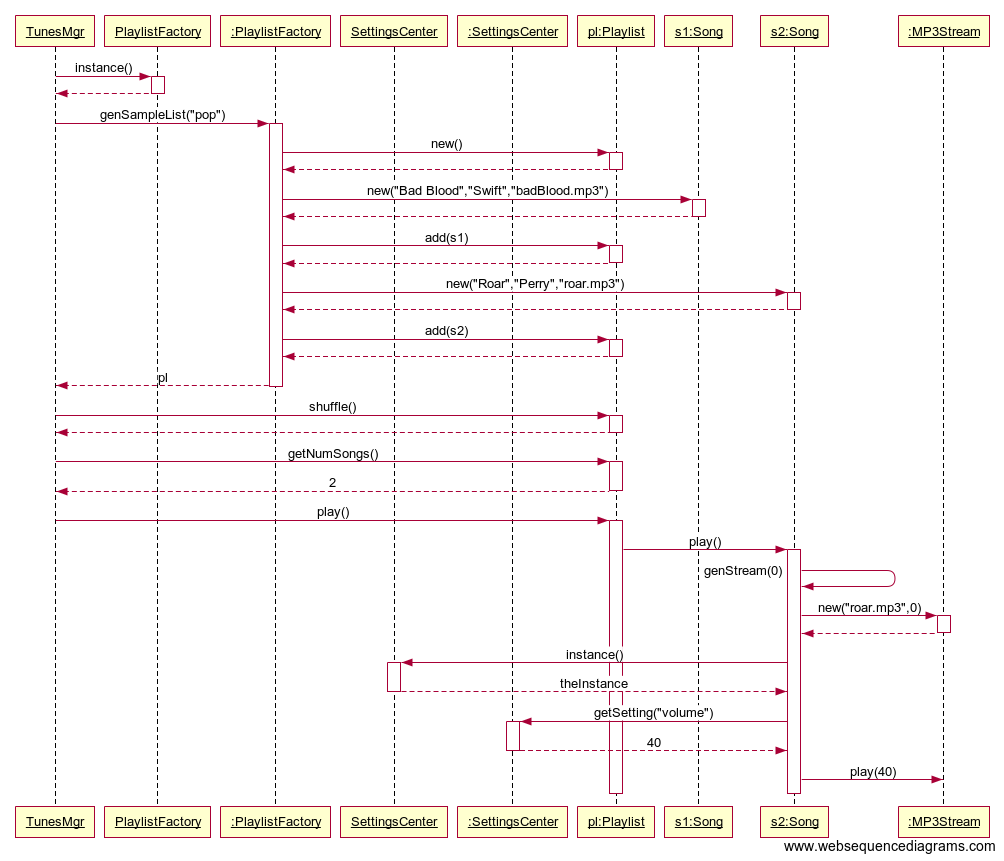
\includegraphics[width=1.25\textwidth]{playlistSeq.pdf}
\vspace{.1in}
\caption{One of the playlist program's sequence diagrams.}
%\quad\quad\quad\quad\quad % hack to center caption
%\protect\phantom{.}}
\label{fig:playlistSeq}
\end{figure}

Here are some things we can read right off the sequence diagram (starting at
the top):

\begin{enumerate}
\itemsep.1em

\item Something in the \texttt{TunesMgr} class will call \texttt{.instance()}
on the \texttt{PlaylistFactory} class. (Notice that the second box from the
left is missing a colon, so it must represent the \textit{class}
\texttt{PlaylistFactory} rather than an object of that type.) Since we're
calling \texttt{.instance()} on a class rather than an object, it had better
be \texttt{static}; and when we look at the class diagram, happily it is.

Furthermore, we can easily guess \textit{which} \texttt{TunesMgr} method is
making that method call, since there's only one listed for it:
\texttt{main()}. After calling \texttt{.instance()} on the class, it looks
like it calls \texttt{.genSampleList("pop")} on the object. Putting it all
together, we can surmise that this code should appear in our
\texttt{TunesMgr.java} file:

\begin{Verbatim}[fontsize=\footnotesize,samepage=true,frame=single]
class TunesMgr {
    public static void main(String args[]) {
        PlaylistFactory pf = PlaylistFactory.instance();
        Playlist p = pf.genSampleList("pop");
        ...to be continued...
    }
}
\end{Verbatim}

All we had to figure out for ourselves was to store the return values in
variables, which seemed like a good idea.

\item Switching scenes to the \texttt{PlaylistFactory}, we get a good sense of
the innards of its \texttt{.genSampleList()} method. The first couple of
arrows coming out of \texttt{:PlaylistFactory} say ``new'', which as you may
guess indicates an \textit{instantiation} and a constructor invocation. In
the first case, we're instantiating a new \texttt{Playlist} object. Apparently
the constructor for \texttt{Playlist} doesn't take any arguments (or the
sequence diagram author didn't bother specifying any). The \texttt{Song}
object we instantiate next, on the other hand, takes a slew of arguments: a
song title, artist, and filename.

After creating this new \texttt{Song}, we \texttt{.add()} it to the
\texttt{Playlist}. We then do the same for another \texttt{Song}. In sum,
here's the kind of thing that \texttt{.getSampleList()} must contain:

\begin{Verbatim}[fontsize=\footnotesize,samepage=true,frame=single]
class PlaylistFactory {
    ...
    Playlist genSampleList(String genre) {
        ...
        Playlist pl = new Playlist();
        Song s1 = new Song("Bad Blood", "Swift", "badBlood.mp3");
        pl.add(s1);
        Song s2 = new Song("Roar", "Perry", "roar.mp3");
        pl.add(s2);
		...
        return pl;
    }
    ...
}
\end{Verbatim}

Now lest we be too hasty, let's step back for a moment. The above code
might well not \textit{literally} be in \texttt{.getSampleList()}; after all,
it refers to specific, hardcoded songs. It also doesn't take into account the
value of \texttt{genre}; presumably, if we passed ``\texttt{rap}'' or
``\texttt{classical}'' as the argument, we'd get a different song selection. So
I'm not actually saying that you can read the code off the diagram without
thinking. What the sequence diagram tells us, though, is good information
about \textit{what kinds of things will happen} in each method. One could
imagine the real \texttt{.getSampleList()} reading song titles from a file or
from an Internet source depending on the genre, for instance. Even in that
case, though, all the sequence diagram essentials would be the same: we'd be
instantiating a new \texttt{Playlist} and \texttt{Song}s, adding the
\texttt{Song}s to the list, \textit{etc.}

\item ``Back to \texttt{main()}!'' the sequence diagram announces. After
returning the \texttt{Playlist} (which Figure~\ref{fig:playlistSeq} suggests
we call ``\texttt{pl}'') our \texttt{main()} method commences calling three
methods on it. We can thus further flesh out our main method as follows:

\begin{Verbatim}[fontsize=\footnotesize,samepage=true,frame=single]
class TunesMgr {
    public static void main(String args[]) {
        PlaylistFactory pf = PlaylistFactory.instance();
        Playlist p = pf.genSampleList("pop");

        p.shuffle();
        int num = p.getNumSongs();
        p.play();
    }
}
\end{Verbatim}

Nothing explicitly told us to save the return value from
\texttt{.getNumSongs()} in a variable, but we did it anyway. We're also not
told what specifically we would do with that information -- perhaps display it
for the user, or estimate the duration of the playlist based on it. At any
rate, for now we'll just save it and move on.

\item Finally, calling \texttt{.play()} on the \texttt{Playlist} turns around
and calls \texttt{.play()} on each of its \texttt{Song}s, not surprisingly. We
can thus deduce something like:

\begin{Verbatim}[fontsize=\footnotesize,samepage=true,frame=single]
public class Song {
    ...
    private ArrayList<Song> songs;
    ...
    public void play() {
        for (Song s: songs) {
            s.play();
        }         
    }
    ...
}
\end{Verbatim}

\item As for \textit{\texttt{Song}'s} \texttt{.play()}
method\footnote{Interestingly, note that there are \textit{three} different
methods called \texttt{.play()} in this design, on each of three different
classes: \texttt{Playlist}, \texttt{Play}, and \texttt{MP3Stream}.}, it
apparently involves calling its own \texttt{.genStream()} method, which in
turn instantiates an \texttt{MP3Stream} object to do the actual playing. After
this, it gets the Singleton \textit{.instance()} from the
\texttt{SettingsCenter} (note that arrows can go right-to-left on sequence
diagrams in addition to left-to-right) and gets the user's \texttt{"volume"}
setting. Finally, it calls \texttt{.play()} on its \texttt{MP3Stream} to play
at the correct volume. Putting it all together, we infer this sort of code:

\begin{Verbatim}[fontsize=\scriptsize,samepage=true,frame=single]
public class Song {
    ...
    public void play() {
        // (the "0" argument means "start at the beginning of the song")
        MP3Stream s = this.genStream(0);  
        int vol = SettingsCenter.instance().getSetting("volume");
        s.play(vol);
    }
    ...
    public MP3Stream genStream(int pos) {
        ...
        return new MP3Stream(this.filename, pos);
    }
}
\end{Verbatim}

Here we choose to chain the calls to \texttt{.instance()} and
\texttt{.getSetting()} rather than saving the \texttt{SettingsCenter} instance
to a variable. This is programmer's discretion. 



\end{enumerate}

Many challenges and questions still remain: how exactly do we go about
generating sample playlists based on genre? What algorithm will
\texttt{.shuffle()} use? Do we play all the songs in a row, back to back, or
do we insert a few seconds of silence in between? How exactly does the
\texttt{MP3Stream} read the bytes off the disk and send them to the audio
speakers? \textit{Etc.} These are important decisions, every bit as important
as what kind of wood and nails to use for each wall we frame. 

But the class diagrams and sequence diagrams have given us a tour of the whole
house as it was envisioned by the architect. We now have a framework into
which all the little decisions can be fit. And that's the first step towards
an elegant and maintainable program.

